\documentclass[11pt,a4paper]{article}
\usepackage[utf8]{inputenc}
\usepackage[english]{babel}
\usepackage{amsmath}
\usepackage{amsfonts}
\usepackage{amssymb}
\usepackage{ragged2e}
\usepackage{graphicx}
\usepackage{float}
\usepackage{hyperref}

\usepackage[left=3cm,right=3cm,top=3cm,bottom=3cm]{geometry}
\begin{document}



\justifying

%%%%%%%%%%%%%%%%%%%%%%%%%%%%%%%%%%%%%%%%%%%%%%%%%%
%%%%%%%%%%%%%%%%%%% TITLE PAGE %%%%%%%%%%%%%%%%%%%
%%%%%%%%%%%%%%%%%%%%%%%%%%%%%%%%%%%%%%%%%%%%%%%%%%

\begin{titlepage}
\begin{center}
{{\Large{\textsc{Motorvehicle University of Emilia-Romagna}}}} \rule[0.1cm]{15.8cm}{0.1mm}
\rule[0.5cm]{15.8cm}{0.6mm}
Master Degree in Advanced Automotive Electronic Engineering

\end{center}

\vspace{15mm}
\begin{center}
{\LARGE{\bf MPC for Dynamic Obstacle Avoidance}}
\rule[0.1cm]{15.8cm}{0.1mm}
\begin{LARGE}

Technical report on the group project activity\\


\end{LARGE}
\vspace{5mm}
Course of Compliance Design of Automotive Systems
\end{center}

\begin{center}
 \begin{figure}[H]
          
\includegraphics[width=1\textwidth]{Figures/MUNER_logo.jpg}
          \end{figure}

 {\large\bf Group memebers:\\}
 {Gianvincenzo Daddabbo}\\
{Gaetano Gallo}\\
{Alberto Ruggeri}\\
{Martina Tedesco}\\
{Alessandro Toschi}\\



\vspace{4mm}
{\large\bf a.y. 2020-2021}
\end{center}
\end{titlepage}

%%%%%%%%%%%%%%%%%%%%%%%%%%%%
%%%%%%%%% Abstract %%%%%%%%%
%%%%%%%%%%%%%%%%%%%%%%%%%%%%

\begin{abstract}
Every year 1.25 million people die and as many as 50 million are injured in road
traffic accidents worldwide, according to United Nations statistics. Human error is involved in about 95\% of all road traffic accidents in the EU, and in 2017 alone, 25,300 people died on the Union’s roads \cite{frisoni2016research}.  
Autonomous cars can improve road safety and through new technologies it is also possible to reduce traffic congestion and CO2 emissions.\\
The aim of this report is to present the steps that we have followed as a group in order to implement a system for dynamic obstacle avoidance using an adaptive Model Predictive Control. 
In the simulated environment, the vehicle model is expected to encounter and safely avoid the dynamic obstacles along its way. 
On the other hand, when an obstacle is not present ahead of the autonomous vehicle, it is expected to follow a predetermined path.

\end{abstract}

\newpage
\tableofcontents
\newpage
\listoffigures
\newpage
\listoftables
\newpage

\section{Introduction}
\label{sec:intro}
\begin{center}
\emph{``Every year 1.25 million people die and as many as 50 million are injured in road
traffic accidents worldwide, according to United Nations statistics. Human error is involved in about 95\% of all road traffic accidents in the EU, and in 2017 alone, 25300 people died on the Union’s roads." \cite{frisoni2016research}}\\
\end{center}
Autonomous cars can improve road safety and through new technologies it is also possible to reduce traffic congestion and CO2 emissions.
The task of avoiding obstacles is one of the key issues when it comes to the vehicular scenario and it is more difficult to perform it here than it is in static environments.
A vehicle with  an obstacles avoidance system is equipped with sensors that measure the distance between the car itself and the obstacle in the same lane. If an autonomous car encounters an obstacle, it is expected to move temporarily to another lane and move back to the original lane once it has driven past the obstacle.
The aim of this report is to present the steps that we have followed as a group in order to implement a system for dynamic obstacle avoidance using an adaptive Model Predictive Control. 
In particular, the report is structured as follows:
\begin{itemize}
    \item the introduction of this report focuses on the basics behind the concepts of Model Predictive Control and Model-Based Design and ends by introducing the software tools used in the project;
    \item starting from Section 2 up to Section 4 we go through the set of requirements of our project laid down by a hypothetical customer, the corresponding low level requirements and the associated validation methods, as well as introducing the system partitioning adopted during the development phase and the mathematical model behind our ego vehicle;
    \item in Section 5 and 6 we go through the various technologies available on the market related to the perception, route planning and control of autonomous vehicles explaining our assumptions regarding these topics. We then proceed explaining how we have imported real maps into our simulation environment and the constraints we have taken into account concerning throttle, steering angle and outputs;
    \item the sections from 7 to 12 are dedicated to the presentation of the actual controller setup and the tests performed in order to validate our controller against the path following task and obstacle avoidance tasks (both static and dynamic, both single and multiple);
   \item the report ends with some considerations on the project carried out and some ideas to further improve it.
\end{itemize}



\subsection{MPC: basic concepts}
In the simulated environment, the vehicle model is expected to encounter and safely avoid obstacles along its way. On the other hand, when an obstacle is not present ahead of the autonomous vehicle, it is expected to follow a predetermined path.
This type of control can be implemented using a Model Predictive Control (MPC).
An MPC is an advanced control method that works in discrete time and uses a model of the system to make predictions about the system’s future behavior. 
Figure \ref{fig:MPC_scheme} graphically shows the general concept behind a Model Predictive Control.
\begin{figure}[H]
    \centering
    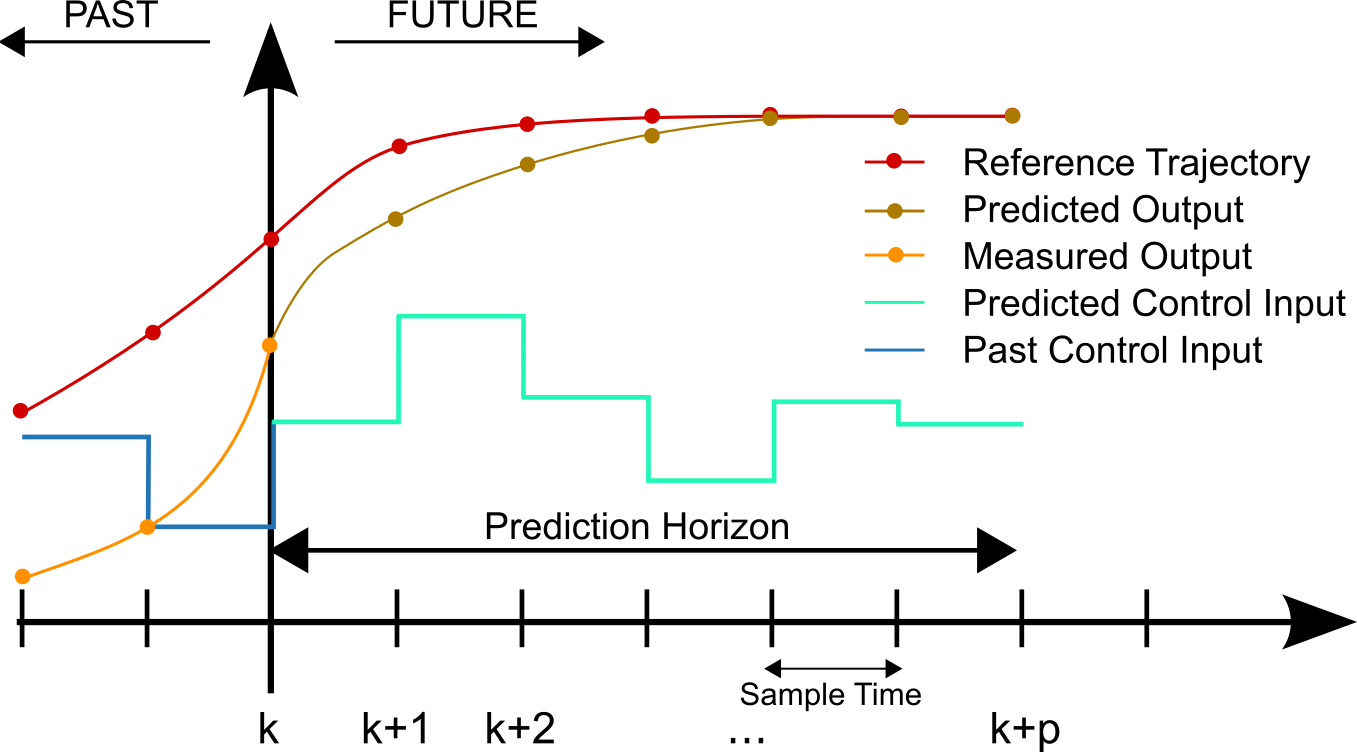
\includegraphics[width=0.9\textwidth]{Figures/MPC_scheme_basic.png}
    \caption{MPC algorithm scheme}
    \label{fig:MPC_scheme}
\end{figure}
The MPC solves an online optimization algorithm to find the optimal control action that drives the predicted output to the reference \cite{MPC_Def}. In other words, from a set of state values, and with respect to a model, it optimizes a problem around an objective and gives a sequence of control signals as outputs. The first set of control values are then used as inputs to the system plant, and after a short period, set as the \emph{system time step}, the new state values are measured and the process is repeated.
The overall objectives of the MPC are:
\begin{itemize}
 

\item prevent that input and output constraints are violated;
\item optimize some input variables, while other outputs are kept in specified ranges;
\item prevent the input variables from having excessive variations.
\end{itemize}
Figure \ref{fig:MPC_Block} shows a block diagram for a Model Predictive Control.
\begin{figure}[H]
    \centering
    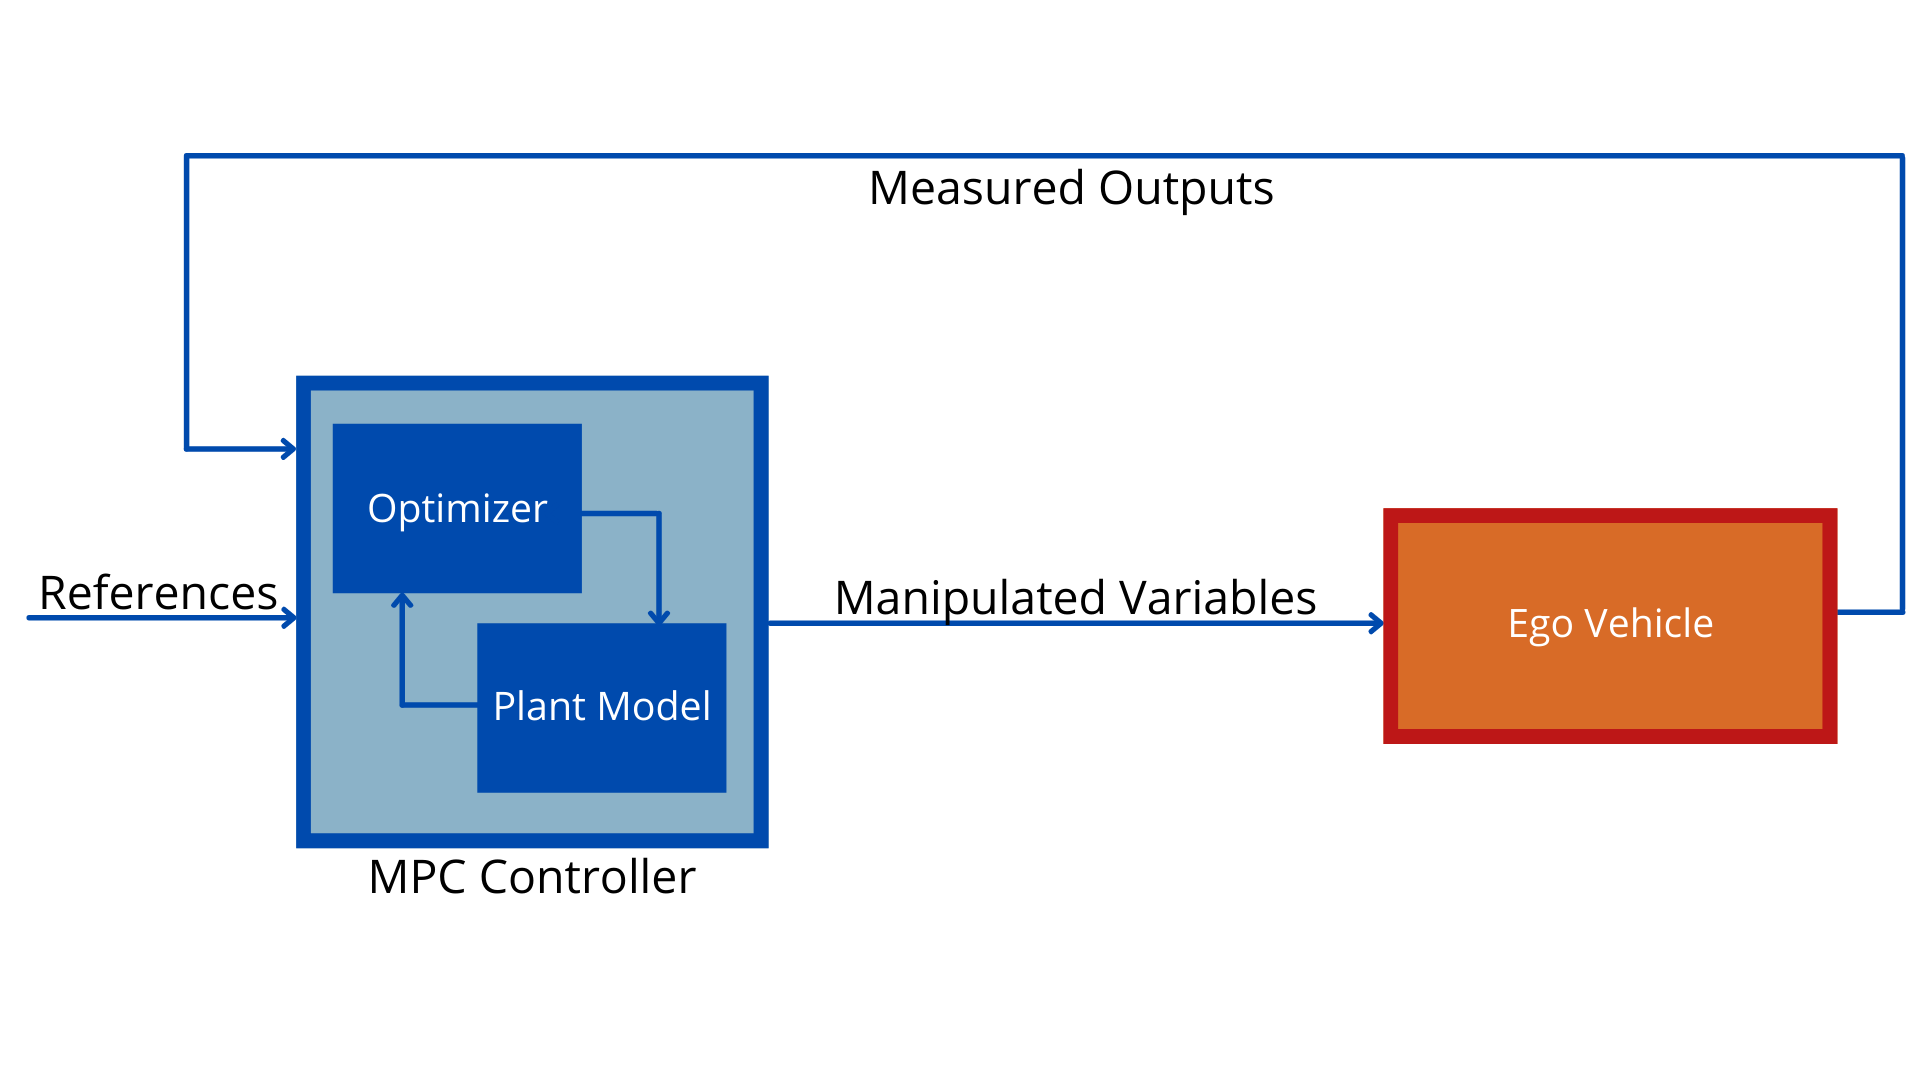
\includegraphics[width=1\textwidth]{Figures/mpcblock.png}
    \caption{MPC Block Diagram}
      \label{fig:MPC_Block}
\end{figure}
An MPC controller has two main functional blocks: the optimizer and the plant model.
The dynamic optimizer allows to find the optimal input that gives the minimum
value of the cost function taking into account all the constraints. Generally, a non linear model is used for the validation of the controller, while the plant model used for the MPC is a linearized version of the actual plant.\\
Our project is based on the use of an \emph{adaptive} MPC, which means that the plant state has to be measured again to be adopted as the linearization point for the next step of the predictive control. When the plant state is re-sampled, the whole process
computes again the calculations starting from the new current state.

\subsection{Model-Based Design}
When developing a project, especially concerning embedded systems, it is crucial to follow a process model which illustrates the high-level activities and their phasing during development.\\
As stated in \cite{FOWLER20151} \emph{``Process models provide high-level perspective that helps team members understand what activities to do and what progress  has been made on each of those development activities"}.\\
The development process of our system is based on the V-model shown in Figure \ref{fig:V_model}.
Starting from the general V-model we have tailored our own V-model in order to meet our needs; doing so we have managed to skip some unnecessary steps in the development process while still being compliant with the definition of the V-model itself.

\begin{figure}[H]
    \centering
    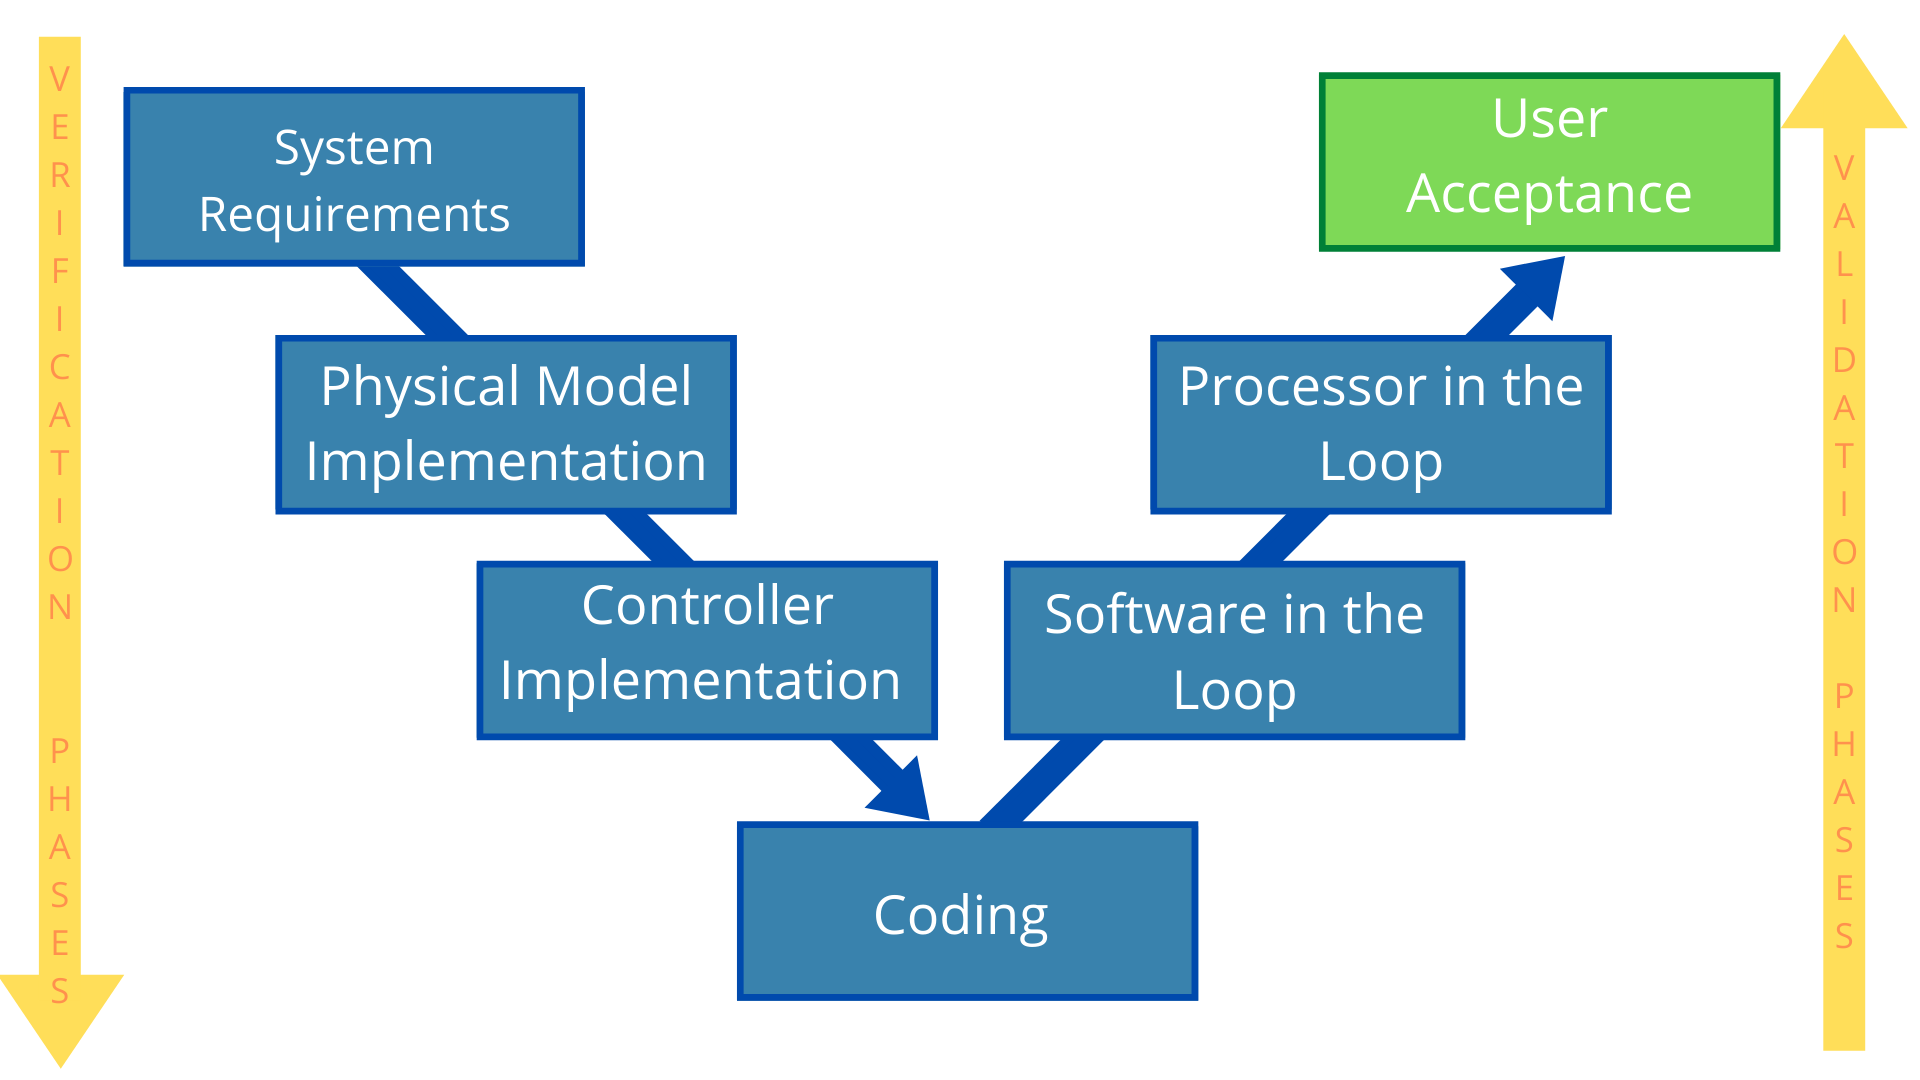
\includegraphics[width=1\textwidth]{Figures/V-MODEL.png}
    \caption{System Development V-model}
    
    \label{fig:V_model}
\end{figure}

As shown above the V-model is a representation of the system development process that highlights verification steps on one side and validation steps on the other of the ``V". The left side of the ``V" identifies the verification phase, containing the steps that lead to code generation while the right side identifies the validation phase which ends with the user acceptance.
Below a brief description of the steps that constitute our V-model:
\begin{itemize}
    \item \textbf{System requirements}: this is the first step of each project, it consists in gathering the requirements from the customer;
    \item \textbf{Physical model implementation}: this phase contains the system design of our vehicle in terms of sensors required and dynamic and kinematic model;
    \item \textbf{Controller implementation}: this phase represents the focus of our project, designing an adaptive MPC;
    \item \textbf{Coding}: exploiting some specific tools, we can automatically generate code for embedded deployment and create test benches for system verification, saving time and avoiding the introduction of manually coded errors;
    \item \textbf{Software-in-the-Loop}: once generated, the code is tested in a simulation environment;
    
    \item \textbf{Processor-in-the-Loop}: during this phase the code is uploaded on a demo board and than it is tested again;
    
    \item \textbf{User Acceptance}: in this phase the final product is tested in order to verify the compliance with the initial costumer requirements.
\end{itemize}

\subsection{Required tools}
The project is based on \href{https://www.mathworks.com/help/matlab/index.html?s_tid=srchtitle}{\underline{MATLAB}}, a proprietary multi-paradigm programming language and numeric computing environment developed by \textit{MathWorks}, and \href{https://www.mathworks.com/help/simulink/index.html?s_tid=CRUX_lftnav}{\underline{Simulink}}, a MATLAB-based block diagram environment for multi-domain simulation and Model-Based Design.\\
The software requirements for the project, including all the applications needed for the proper execution and test are listed below:
\begin{itemize}
    \item \textbf{MATLAB R2019a or newer};
    \begin{enumerate}
            \item \textbf{Curve Fitting Toolbox}: needed to make the reference map smoother;
            \item \textbf{Automated Driving Toolbox}: needed to import a reference map from real world data;
            \item \textbf{Model Predictive Control Toolbox}: needed to have all the useful resources to develop the MPC.
    \end{enumerate}
    \item \textbf{Simulink 9.3 or higher};
    \begin{enumerate}
            \item \textbf{Simulink Test}: used to perform automated tests and requirements verification;
            \item \textbf{Embedded Coder}: used for automatic code generation.
    \end{enumerate}
    
    \item \textbf{STM32CubeMx}: needed to define the peripheral configuration;
    \item \textbf{STM32CubeIDE}: used to build the generated code and load it on the target board;
    \item \textbf{STM32-MAT}: extension used to run Simulink applications models on STM32 MCUs.
\end{itemize}

As it will be discussed later on in Section \ref{subsection:PIL}, the last three tools are required for the PIL simulation since we have used a STM32 microcontroller.





\section{System Requirements} \label{System_Requirements}


Defining the project requirements is an essential and crucial step to accomplish in the starting phase of the project. Indeed, from both the perspective of the customer and of the project developers, detailed requirements are necessary to deliver exactly what is needed.\\
Firstly, the requirements are defined by the customer at a high level, then ``translated" by the developers to a lower and technical level and later on validated to ensure that the project requirements are correct, free of defects/bugs, and meet the needs of the users.\\
For the sake of this project we have assumed to receive the requirements from a hypothetical customer.
Namely, there are six high level requirements given for this obstacle avoidance implementation that are mainly related to the accuracy of the system and to the driver comfort:
\begin{enumerate}
    \item maximum lateral error from reference of 0.75 $m$;
    \item detection of obstacles within 100 $m$ ahead of the vehicle;
    \item move on left lane within a predetermined safe zone from the obstacle\footnote{Third and fourth requirement are requested when an obstacle is detected.};
    \item once the obstacle has been passed, come back on the right lane at no less than 10 $m$ but no more than 50 $m$ ahead of it;
    \item maximum lateral acceleration of 2 $m/s^2$;
    \item all previous requirements satisfied in the speed range from 10 $km/h$ to 100 $km/h$.
\end{enumerate}

%\include{Chapters/Sensors}
%\include{Chapters/SafetyDistance}






\newpage
\bibliography{Compliance.bib}
\bibliographystyle{unsrt}

\end{document}  
